
\section{Theorie}
\label{sec:Theorie}

\subsection{Die Kathodenstrahlröhre}

Die Kathodenstrahlröhre besteht aus einem Erzeugungs-, einem Ablenk- und einem Nachweissystem.
Das Erzeugungssystem erzeugt einen fokussierten Elektronenstrahl, indem durch Glühemission aus einer Kathode freie Elektronen emittiert werden. Die Kathode ist von einem Wenelt-Zylinder mit negativem Potential umgeben, welcher in Strahlrichtung eine Öffnung besitzt, sodass die Intensität des Elektronenstrahls gesteuert werden kann.
Nach dem Wenelt-Zylinder werden die übrig gebliebenen Elektronen durch eine positiv geladene Elektrode mit einer Beschleunigungsspannung $U_.B$ beschleunigt und anschließend durch weitere Elektroden mithilfe inhomogener Felder fokussiert.\\
Hinter dem Erzeugungssystem befindet sich das Ablenksystem, welches aus zwei orthogonal zueinander stehenden Plattenpaaren besteht, deren Abstand $d$ klein gegenüber der Plattenlänge $p$ ist. Zwischen den Platten wird somit mithilfe einer Ablenkspannung $U_.d$ ein nahezu homogenes elektrisches Feld $E$ der Form
\begin{equation}
E = \frac{U_d}{d}\label{eq:E}
\end{equation} 
erzeugt, welches die Elektronen senkrecht zur Strahlrichtung beschleunigt, sodass sie aus ihrer ursprünglichen Bahn abgelenkt werden.\\
Nach dem Ablenksystem trifft der Elektronenstrahl auf das Nachweissystem, welches aus einem Leuchtschirm besteht. Durch die einfallenden Elektronen wird dieser an den Auftreffpunkten zur Emission von Lichtquanten angeregt, sodass der Elektronenstrahl am Schirm sichtbar gemacht wird. Um eine Aufladung des Schirmes durch die Elektronen zu vermeiden, ist er elektrisch mit der Beschleunigungselektrode verbunden. Ein Schema des Aufbaus der Kathodenstrahlröhre ist in Abbildung \ref{fig:Kathodenstrahlröhre} zu sehen.   

\begin{figure}
\centering
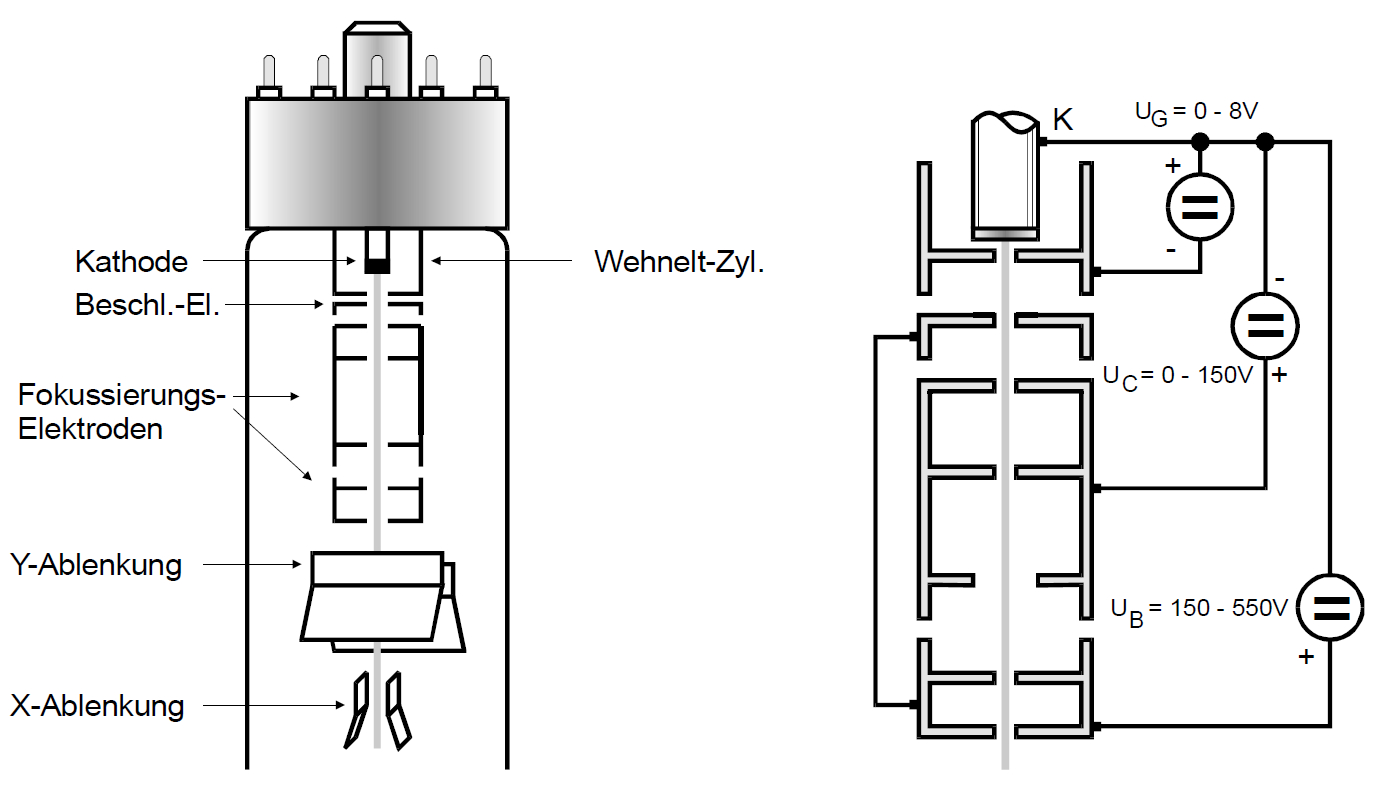
\includegraphics[width=\linewidth-50pt,height=\textheight-50pt,keepaspectratio]{content/images/Kathodenstrahlroehre.jpg}
\caption{Der Schematische Aufbau einer Kathodenstrahlröhre und die Beschaltung des Erzeugungssystems \cite{V501}.}
\label{fig:Kathodenstrahlröhre}
\end{figure}

\subsection{Ablenkung des Elektronenstrahls im elektrischen Feld und der Kathodenstrahloszillograph}

Wie bereits im vorherigen Abschnitt beschrieben, werden die Elektronen im elektrischen Feld beschleunigt, es wirkt also eine Kraft $F$. Mit Formel \eqref{eq:E} kann diese beschrieben werden durch:
\begin{equation}
F_.{el} = e_0E = e_0\frac{U_.d}{d}\text{.}\label{eq:F_el}
\end{equation}  
Dabei stellt $e_0$ die Elementarladung des Elektrons mit Masse $m_e$ dar. Da die Kraft in Formel \eqref{eq:F_el} konstant ist, handelt es sich um eine gleichmäßig beschleunigte Bewegung und die Geschwindigkeit $v_.y$ der Elektronen in Ablenkrichtung beträgt nach dem Beschleunigungsvorgang:
\begin{equation}
v_.y = \frac{F_.{el}}{m_e}\Delta t = \frac{e_0U_.d}{m_ed}\frac{p}{v_.z}\text{.}\label{eq:vy}
\end{equation}
$\Delta t$ ist die Zeitdauer, in welcher die Elektronen beschleunigt werden, $v_.z$ ist die Geschwindigkeit, welche die Elektronen bei Eintritt in das Feld besitzen. Wegen der Energieerhaltung hängt diese von der Beschleunigungsspannung ab:
\begin{equation}
v_.z^2 = \frac{2e_0U_.B}{m_e}\text{.}\label{eq:vz}
\end{equation}
Für die Verschiebung $D$ des Leuchtfleckes am Schirm ergibt sich also mit den Formeln \eqref{eq:vy} und \eqref{eq:vz}:
\begin{equation}
D = L\frac{v_.y}{v_.z} = \frac{p}{2d}L\frac{U_.d}{U_.B}\text{.}\label{eq:D}
\end{equation}   
Dabei beschreibt $L$ den Abstand der Ablenkplatten zum Leuchtschirm (vergleiche Abbildung \ref{fig:E-Feld}).

\begin{figure}
\centering
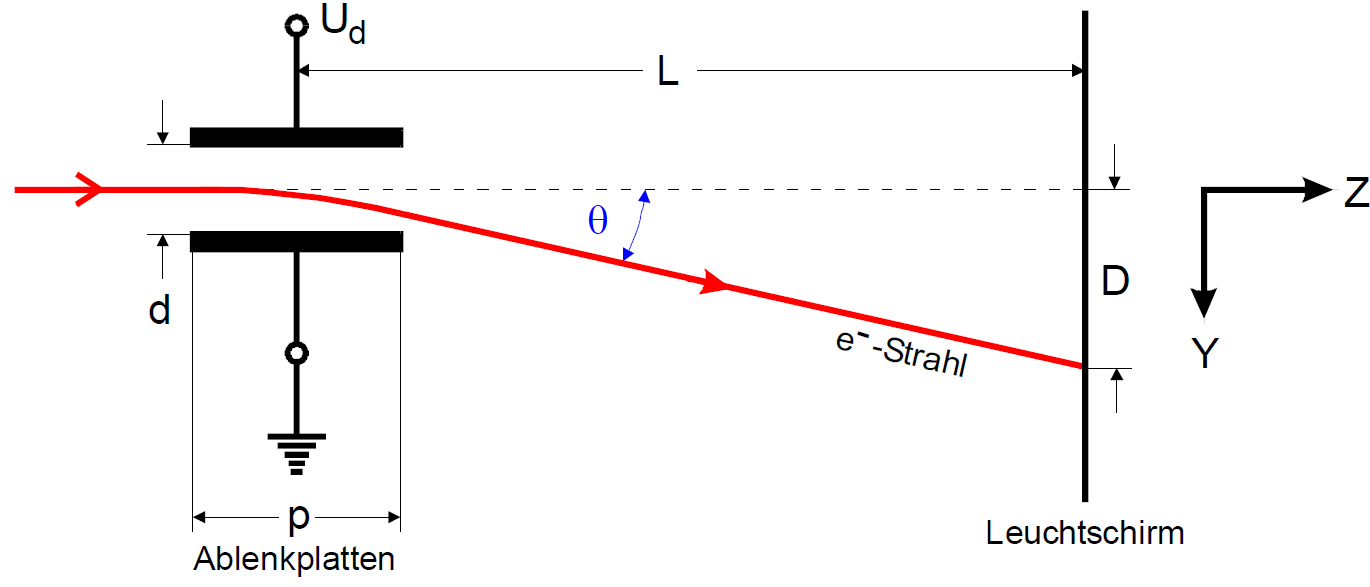
\includegraphics[width=\linewidth-50pt,height=\textheight-50pt,keepaspectratio]{content/images/Ablenkung-Im-E-Feld.jpg}
\caption{Schema zur Beschreibung der Ablenkung im elektrischen Feld \cite{V501}.}
\label{fig:E-Feld}
\end{figure}

\noindent Wird an die horizontal ablenkende Platte eine Sägespannung angelegt, so kann die Kathodenstrahlröhre als Oszillograph verwendet werden, indem an die vertikal ablenkende Platte die zu untersuchende Wechselspannung angelegt wird.
Der zeitliche Verlauf der zu untersuchenden Spannung kann nur dann als stehendes Bild dargestellt werden, wenn das Verhältnis der Frequenz der Sägespannung $f_.S$ und der Wechselspannung $f_.W$ wie folgt aufeinander abgestimmt ist:
\begin{equation}
nf_.S=mf_.W\text{ ;}n,m\in \mathbb{N}\text{.}\label{frequenzabhängigkeit}
\end{equation}

\subsection{Ablenkung des Elektronenstrahls im magnetischen Feld und Bestimmung der spezifischen Ladung des Elektrons}

Bewegt sich ein Elektron mit der Geschwindigkeit $\vv{v}$ in einem magnetischen Feld $\vv{B}$, so wirkt auf es die Lorentzkraft:
\begin{equation}
\vv{F}_.L = e_0\vv{v}\times\vv{B}\text{.}\label{eq:Lorenz}
\end{equation}
Es wirkt demnach nur eine Kraft auf das Elektron, wenn es eine Geschwindigkeitskomponente senkrecht zum Magnetfeld besitzt.
Besitzt das Elektron nur eine konstante Geschwindigkeitskomponente $v_0$ senkrecht zum Magnetfeld, so wird es in einer Kreisbahn abgelenkt. Dies folgt aus der Energieerhaltung, da das Elektron eine konstante kinetische Energie besitzt. Für den Radius $r$ dieser Kreisbahn ergibt sich nach Gleichsetzen der Zentrifugalkraft mit der Lorentzkraft aus Formel \eqref{eq:Lorenz}:
\begin{equation}
r = \frac{m_ev_0}{e_0B}\text{.}\label{eq:r}
\end{equation}
Mithilfe von Formel \eqref{eq:r} und einer Kathodenstrahlröhre kann die spezifische Ladung $\frac{e0}{m0}$ bestimmt werden. Dabei wird $v_0$ analog zu $v_.z$ wie in Formel \eqref{eq:vz} bestimmt.
Da am Leuchtschirm nur der Abstand $D$ gemessen werden kann, wird mit Abbildung \ref{fig:B-Feld} folgende Beziehung zwischen $r$ und $D$ hergeleitet:
\begin{equation}
r = \frac{L^2+D^2}{2D}\text{.}\label{eq:r2}
\end{equation}
Dabei ist $L$ der Wirkungsbereich des magnetischen Feldes. Nach Gleichsetzen von Formel \eqref{eq:r} und \eqref{eq:r2} ergibt sich mit einsetzen von $v_0$ für die spezifische Ladung:
\begin{equation}
\frac{e_0}{m_e} = \frac{8U_.BD^2}{(L^2+D^2)^2B^2}\text{.}\label{eq:e0/me}
\end{equation}

\begin{figure}
\centering
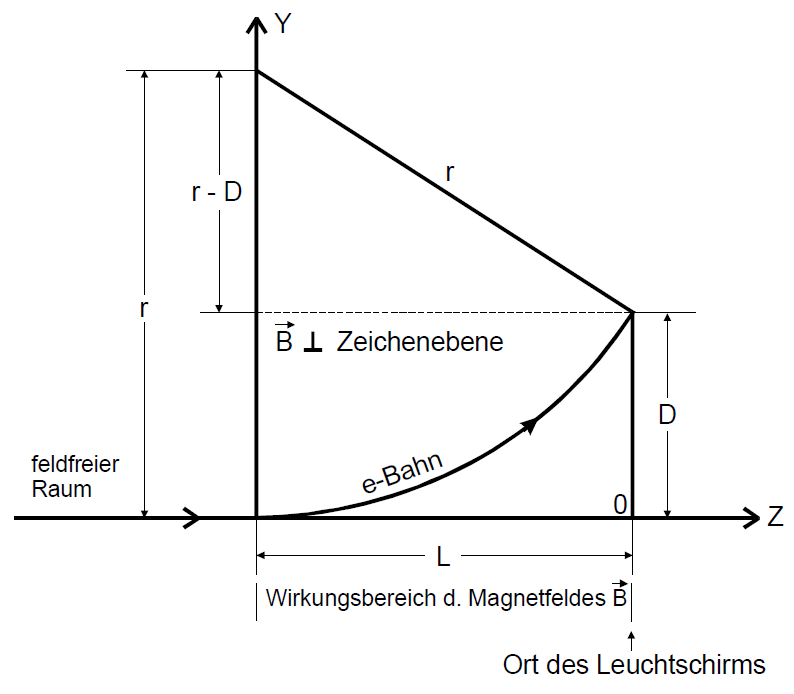
\includegraphics[width=\linewidth-70pt,height=\textheight-70pt,keepaspectratio]{content/images/Ablenkung-Im-B-Feld.jpg}
\caption{Schema zur Beschreibung der Ablenkung im magnetischen Feld \cite{V502}.}
\label{fig:B-Feld}
\end{figure}